\Chapter{Times Remembered}{Clare Court}

In the course of writing any part of this account, which originally began as a straightforward description of our experiences on taking over the family business, I became more and more involved in the early history of our home and the people who built it. Gradually the story moved as it were out of my own hands and I found the subject matter leading backwards in time of its own volition, through the forties to the years before my birth. I must confess unashamedly, that if anyone had asked me when we first conceived the idea of writing this book who were to be the most important characters in it, I would have said Glyn and myself. As the tale progressed however, it became increasingly obvious that the real hero and heroine were not ourselves but Glyn's parents, William and Ada. Little by little and bit by bit, I started to put together all the many pieces of information which I had unwittingly collected over the years - the oft-repeated tales to which one listened oh so reluctantly, twenty or so years ago.

One has mixed memories of the time when all this information was so unwillingly received. When I first came to Washford and though older members of the family were still alive, the traditional time for getting together around the fire, in fact almost the only time free from other interruptions, was Sunday evening after service at the chapel - a sore deprivation to us, the pampered, over-educated and intolerant young, who would have much preferred to listen to a nice concert on the radio or read our books.

William and Ada always attended evening service at the home chapel of Roadwater, and this was generally the highlight of the week for them as it was the only time they were able to spend with his sister and any other members of the family who happened to be visiting. The meeting place was in one of the cottages, which adjoined the widest part of the road through the village - the Bridge, as it is always known. This area, though hardly meriting the description of “square”, served very well in the past as the hub and focal point of village life. Roadwater straggles along the cleft of a steep and narrow valley which is overhung by dark trees, so whichever house was chosen it was certain that very little daylight would illumine the proceedings. There was no escape as we dutifully filed into the tiny cramped, room smelling of mothballs and paraffin lamps - except for Glyn who would delay his appearance round the tea pot for a considerable time by lingering at the keyboard of the organ. His parents were very proud of his playing and never protested if the practice went on for a goodish spell. There is a certain finesse in doing what one wants to do without upsetting the older generation, and as an adolescent he had perfected, the art of disappearing when unpleasant or boring tasks seemed imminent. He tells me that he used frequently to retreat to the small copse which stands up the hill at the top of our garden, and there, safely out of earshot of the house and away from the continual annoyance of telegrams, he would, truthfully claim that he had not heard his parents when they called him. In this quiet spot he read his way through a good many books, including most of the plays of Racine. The copse, though less secluded now than at the time of which I am writing, is an embowered, spot overlooking the Abbey, though perhaps more suited, to the reading of romantic poetry than of seventeenth century tragedy. There is a piquancy, though, in the contrast between our homely scene and the stately characters of those long dead. Kings and Queens fighting out their battles of love and hate in beautifully measured Alexandrines, which I find, particularly appealing!

I, however, had no excuse to linger, and not being a rebel by nature would have found it difficult to hurt the feelings of my kindly parents-in-law. For I had so much to learn, and the code of behaviour which was expected from me was not one of which I had any previous experience and demanded my full attention. Their way of life, based on Methodism, was ruled by what seemed to me strange habits and taboos, as alien to me as the customs of some foreign tribe. For example, when I was first welcomed into the family I found it difficult to understand why l must never mention alcoholic drink of any sort, let alone disclose the terrible fact that my family regularly brewed home-made wine. Playing cards (the \quotemark{devil's pictures} to an older generation) were also a forbidden subject, and I had to remember not to mention that we often played bridge and whist at home - for buttons never money, as there were some taboos even in my family. The vocabulary too puzzled me. Temperance, a word which was constantly on their lips, did not seem to mean what I thought it meant but it was not long before I came to realise that its true meaning was Total  Abstinence in the particular context of the flourishing local nineteenth century Temperance Movement. All the men of the family had signed the Pledge and this too was frequently spoken of, but no one seemed to think it necessary to explain to me what was meant.

So there we sat, eating our bread and butter and drinking our tea from the carefully preserved china tea service with pink handles that was brought out on these occasions. And then the reminiscences would begin. Stories, incidents, biographies of long-dead friends, memories of childhood recalled in all the circumstantial detail - all these and more were repeated time and time again on those Sunday evenings. The tale would unfold like a symphony, beginning generally with a theme by William, the conductor of the orchestra. As he developed it the other members of the gathering would offer their contributions or develop a theme of their own at a given signal from the leader, and gradually the exposition would come, rise to its climax and finally subside to its logical and expected conclusion. As the years passed and I became familiar with certain stories I came to know the effect that certain words and phrases would have, for the same situations would provoke the same reminiscences. For example, whenever any ironing was being done, Ada would very easily launch into a little tale about her sister Florrie who once kept house for a lady who did not believe in ironing her underclothes. With experience, I came to learn how to steer the conversation gently away from this not particularly interesting subject. Garden herbs and sage in particular always reminded Ada of her childhood, so that if stuffing was being made I came to expect an oft repeated account of the making of faggots from the freshly killed pig at her cottage home in Lydney. The faggots probably tasted delicious - though I fancy they used to put in too much sage for my taste.

I realise now, though at the time I did not, as I listened to all these tales and shared the simple refreshment with my husband's family that I was hearing the swansong of the last generation in modern times who relied to a very large extent on the spoken oral tradition word to transmit their history from one generation to the next.

I can see now that the continual repetition of the same information was an essential part of the tradition, for only in this way would the proper continuance of the story be ensured. Besides, the oldest stories were the ones that were loved the best, and every repeat performance evoked happy memories of the past. It is not in my province to say whether the older stories changed much as they came down through the years. All the evidence that we have of such matters would point to the fact that they did. As none of us was present at the original events it is obviously impossible no to prove or disprove anything - but it is quite beyond dispute that however much variation there might be in detail the facts were based on true happenings. Some of these tales, which Glyn will be recounting in another place, originated in a most astonishing assortment of subjects. Birth, death, childhood reminiscences, the soil, a liberal sprinkling of humour, some coarse (though these versions were never considered fit for my ears), religious experiences - and always lurking round the corner, his forked tail visibly twitching - the devil. There is one of these tales which even now after I have heard it so many times, chills my spine to the marrow.
 
\begin{figure}
     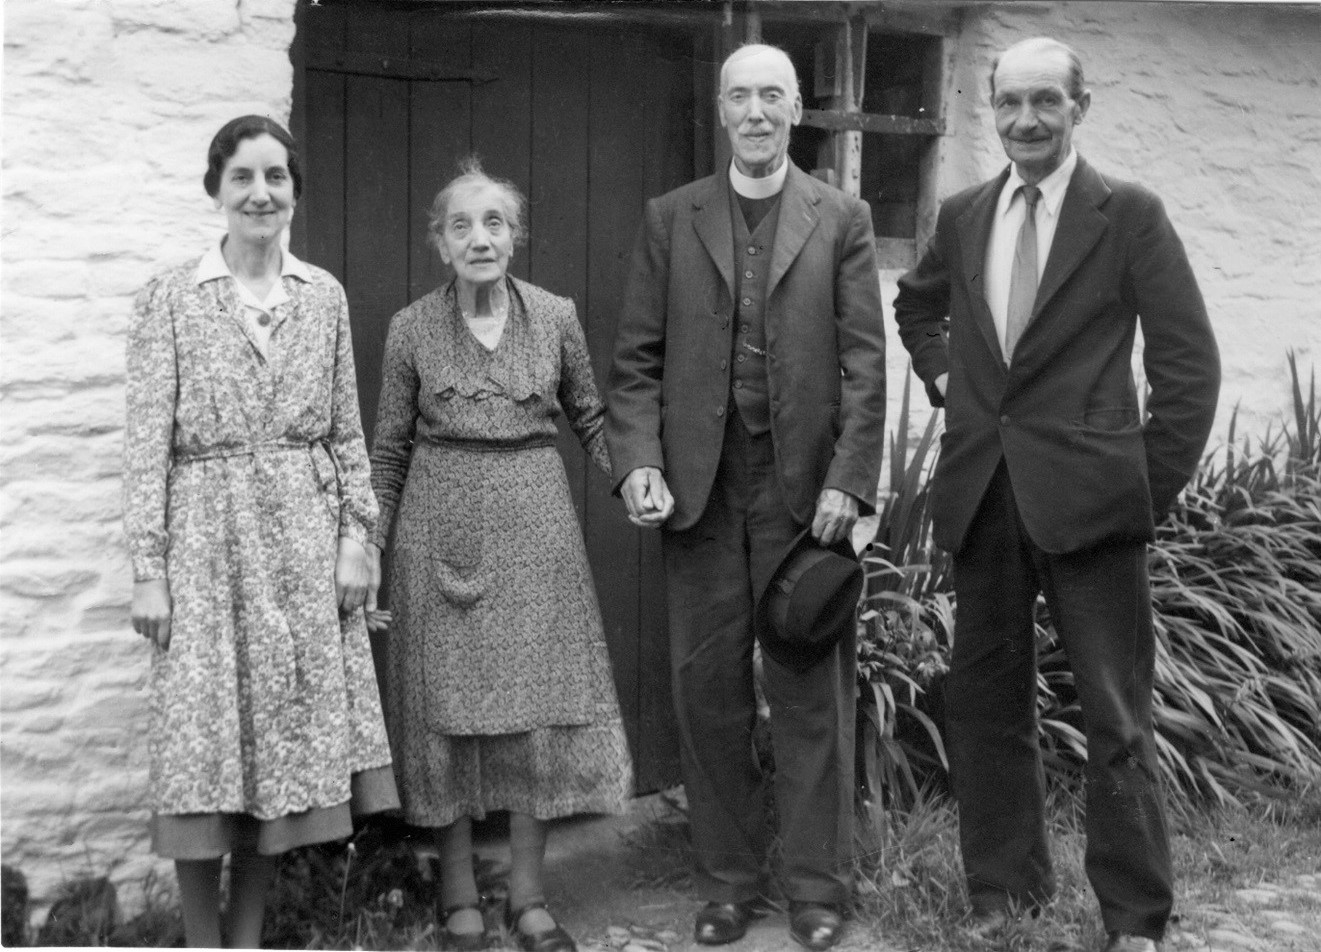
\includegraphics[width=1\textwidth]{figures/familyPhoto}
     \caption{Kathie, Selina, Lewis and Walter}
     \label{fig:Family}
\end{figure}

Dear William, Ada, Selina, Lily, Lewis and Walter! It would be easy to scoff at the regularity of your lives, and the satisfaction and contentment which such a simple evening's entertainment gave you, but like so many things which exist no longer, it is only quite recently that we have come to learn the value of what you said. Believe it if you can - but I find myself trying, often unsuccessfully, to remember some of those conversations. Perhaps you will forgive me though if I tell you that I am not the only person who did not listen properly to what you used to say. Even Kathie, who is over 70, tells me that she too paid little attention to your stories, Selina, and it was only with some perseverance that I was able to find out a few details of your life. And even Glyn does not remember many of the sayings that I seem to have retained. He admits that he used to switch off whenever the \quotemark{old days} were being discussed.

To return to the subject of William and Ada unconsciously taking over the book. If they were alive today they would be very surprised indeed to learn that anyone could possibly be interested in their lives and work.

Poor William struggled with an inferiority complex all his life, convinced as he was of the superior ability and success of his elder brother Lewis. True, Lewis had done well for after educating himself he had become an ordained minister in the Methodist church, William too had longed to enter the ministry but there were obstacles in the way of achieving his heart’s desire. For one thing his health as a young man was not good, and even when this improved he had taken on the further burden of bringing up his sister's children. Then there was the necessity of learning Greek, Not surprisingly classical languages had not been included in the curriculum at the tiny Leighland school and even if they had, William would have had little time to learn them, leaving as he did at the tender age of twelve. Frustrated but not totally daunted by his lack of education, he did his best to make up for it in later years. The whole of his creative talent, which was considerable, was poured into his life. The great loves of his life, apart from the chapel and all its activities were music, woodcarving, the countryside and its history. The high point of his achievement, were the building of his own house and the creation of the garden, and I now propose to set down as accurately as I am able, the history of its construction.